
\includepdf[templatesize={210mm}{350mm}, noautoscale=true, scale=0.9, pages=1, pagecommand=\section{Information till lärare}]{Appendix/Info/AllmanInfoLarare.pdf}
    \label{app:info}

%\section{Den fullständiga versionen av problemen}
    %\subsection{Fermiproblem}
    %\includepdfmerge[nup=2x2] {Appendix/Problem/Fermi.pdf, 1-4}
    
\includepdf[templatesize={210mm}{390mm}, noautoscale=true, pages=1, scale=1, pagecommand=\section{Den fullständiga versionen av problemen}\subsection{Fermiproblem}\label{app:problemen}]{Appendix/Problem/Fermi.pdf}
    
\includepdf[pages=2]{Appendix/Problem/Fermi.pdf}
    
\includepdf[pages=3]{Appendix/Problem/Fermi.pdf}
    
\includepdf[pages=4]{Appendix/Problem/Fermi.pdf}
    
    %\subsection{Flygplan}
    
\includepdf[pages=1, templatesize={210mm}{370mm}, noautoscale=true, pages=1, scale=1, pagecommand=\subsection{Flygplan}]{Appendix/Problem/Flygplan.pdf}
    
\includepdf[pages=2]{Appendix/Problem/Flygplan.pdf}
    
\includepdf[pages=3]{Appendix/Problem/Flygplan.pdf}
    
\includepdf[pages=4]{Appendix/Problem/Flygplan.pdf}
        
    %\subsection{Fritt fall}
    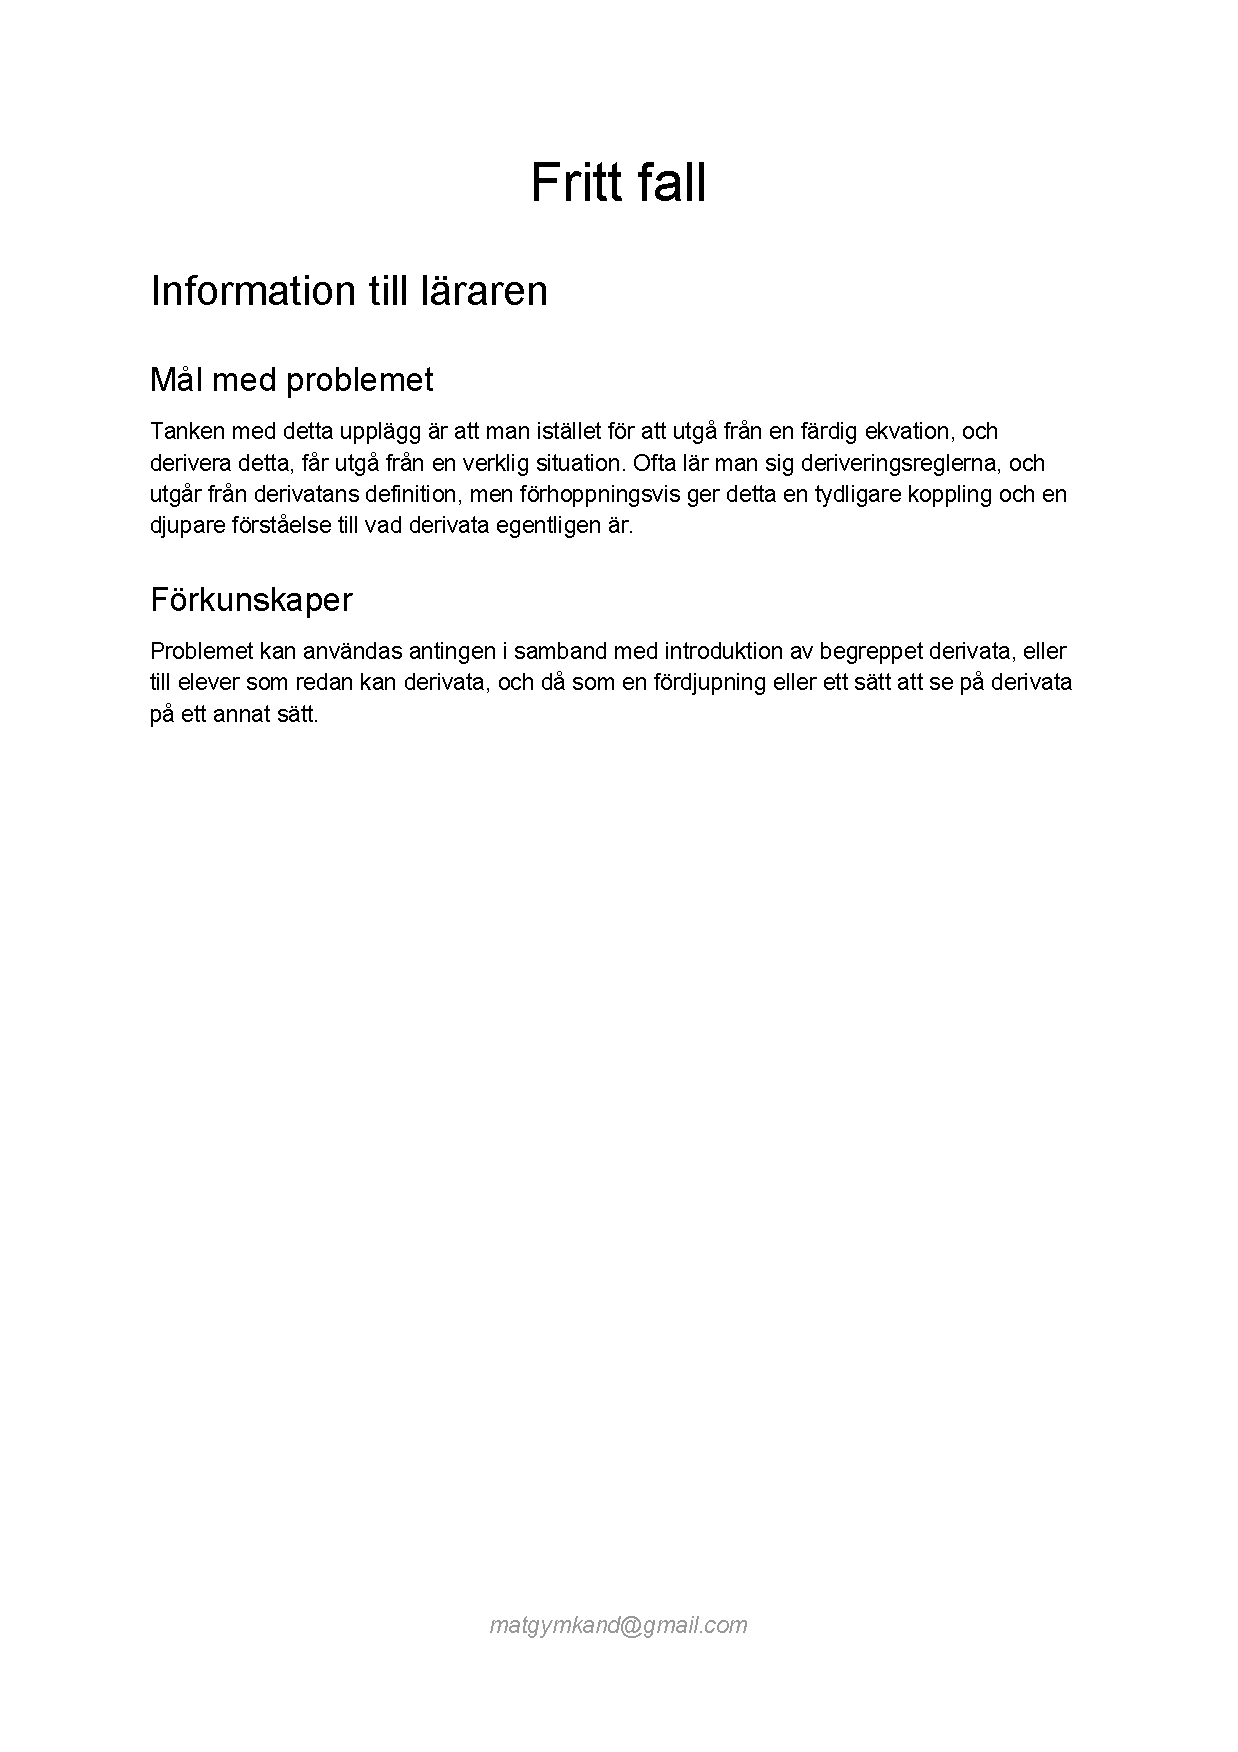
\includepdf[pages=1, templatesize={210mm}{370mm}, noautoscale=true, pages=1, scale=1, pagecommand=\subsection{Fritt fall}]{Appendix/Problem/Frittfall.pdf}
    \includepdf[pages=2]{Appendix/Problem/Frittfall.pdf}
    \includepdf[pages=3]{Appendix/Problem/Frittfall.pdf}
    
    %\subsection{Försvåring av en ekvation}
        %\includepdfmerge[nup=2x2] {Appendix/Problem/Ekvation.pdf, 1-4}
    
\includepdf[pages=1, templatesize={210mm}{370mm}, noautoscale=true, pages=1, scale=1, pagecommand=\subsection{Försvåring av en ekvation}]{Appendix/Problem/Ekvation.pdf}
    
\includepdf[pages=2]{Appendix/Problem/Ekvation.pdf}
    
\includepdf[pages=3]{Appendix/Problem/Ekvation.pdf}
    
\includepdf[pages=4]{Appendix/Problem/Ekvation.pdf}
    
    %\subsection{Matematisk modell för bil och löpare}
    %    \includepdfmerge[nup=2x2] {Appendix/Problem/Lopare.pdf, 1-3}
    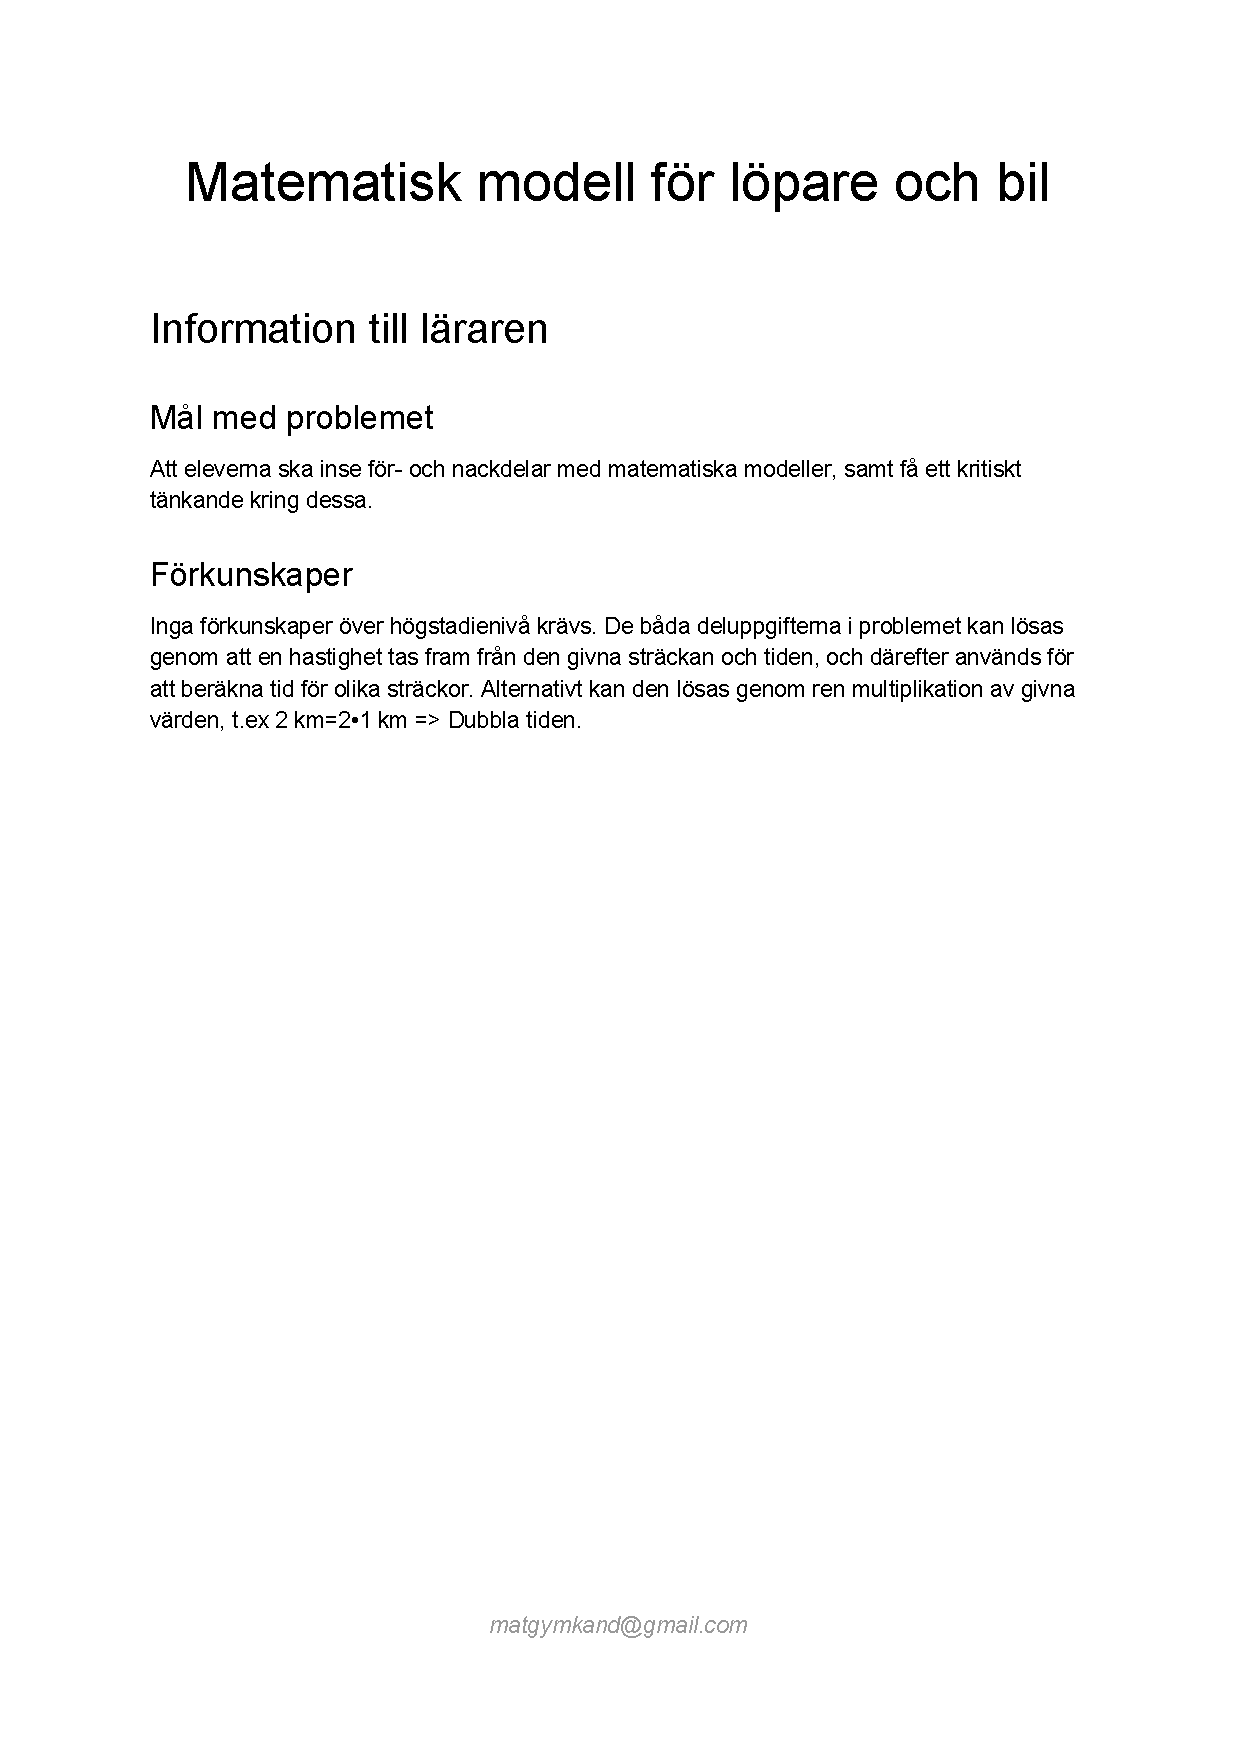
\includepdf[pages=1, templatesize={210mm}{370mm}, noautoscale=true, pages=1, scale=1, pagecommand=\subsection{Matematisk modell för bil och löpare}]{Appendix/Problem/Lopare.pdf}
    \includepdf[pages=2]{Appendix/Problem/Lopare.pdf}
    \includepdf[pages=3]{Appendix/Problem/Lopare.pdf}
    
    %\subsection{Sortera en kortlek}
        %\includepdfmerge[nup=2x2] {Appendix/Problem/Sortera.pdf, 1-4}
    
\includepdf[pages=1, templatesize={210mm}{340mm}, noautoscale=true, pages=1, scale=1, pagecommand=\subsection{Sortera en kortlek}]{Appendix/Problem/Sortera.pdf}
    
\includepdf[pages=2]{Appendix/Problem/Sortera.pdf}
    
\includepdf[pages=3]{Appendix/Problem/Sortera.pdf}
    
\includepdf[pages=4]{Appendix/Problem/Sortera.pdf}
    
    %\subsection{Sorteringsalgoritmer}
    
\includepdf[pages=1, templatesize={210mm}{370mm}, noautoscale=true, pages=1, scale=1, pagecommand=\subsection{Sorteringsalgoritmer}]{Appendix/Problem/Prog/Sorteringsalgoritmer.pdf}
    
\includepdf[pages=2]{Appendix/Problem/Prog/Sorteringsalgoritmer.pdf}
    
\includepdf[pages=3]{Appendix/Problem/Prog/Sorteringsalgoritmer.pdf}
    
    %\subsection{Approximera ett irrationellt tal}
    
\includepdf[pages=1, templatesize={210mm}{370mm}, noautoscale=true, pages=1, scale=1, pagecommand=\subsection{Approximera ett irrationellt tal}]{Appendix/Problem/Prog/Irrationellatal.pdf}
    
\includepdf[pages=2]{Appendix/Problem/Prog/Irrationellatal.pdf}
    
\includepdf[pages=3]{Appendix/Problem/Prog/Irrationellatal.pdf}   
    %\subsection{Fibonaccis talsekvens}
    
\includepdf[pages=1, templatesize={210mm}{370mm}, noautoscale=true, pages=1, scale=1, pagecommand=\subsection{Fibonaccis talsekvens}]{Appendix/Problem/Prog/Fibonacci.pdf}
    
\includepdf[pages=2]{Appendix/Problem/Prog/Fibonacci.pdf}
    
\includepdf[pages=3]{Appendix/Problem/Prog/Fibonacci.pdf}
    
    %\subsection{Identifiera primtalsfaktorer}
    
\includepdf[pages=1, templatesize={210mm}{370mm}, noautoscale=true, pages=1, scale=1, pagecommand=\subsection{Identifiera primtalsfaktorer}]{Appendix/Problem/Prog/Primtalsfaktorer.pdf}
    
\includepdf[pages=2]{Appendix/Problem/Prog/Primtalsfaktorer.pdf}
    
\includepdf[pages=3]{Appendix/Problem/Prog/Primtalsfaktorer.pdf}
    
    %\subsection{Personnummer}
    
\includepdf[pages=1, templatesize={210mm}{370mm}, noautoscale=true, pages=1, scale=1, pagecommand=\subsection{Personnummer}]{Appendix/Problem/Prog/Personnummer.pdf}
    
\includepdf[pages=2]{Appendix/Problem/Prog/Personnummer.pdf}
    
\includepdf[pages=3]{Appendix/Problem/Prog/Personnummer.pdf}
    
\includepdf[pages=4]{Appendix/Problem/Prog/Personnummer.pdf}
    
    %\subsection{Skapa ett chiffer}
    
\includepdf[pages=1, templatesize={210mm}{370mm}, noautoscale=true, pages=1, scale=1, pagecommand=\subsection{Skapa ett chiffer}]{Appendix/Problem/Prog/Chiffer.pdf}
    
\includepdf[pages=2]{Appendix/Problem/Prog/Chiffer.pdf}
    
\includepdf[pages=3]{Appendix/Problem/Prog/Chiffer.pdf}
    
\includepdf[pages=4]{Appendix/Problem/Prog/Chiffer.pdf}

\newpage    

%\section{Presentationerna tillhörande problemen}
    %\subsection{Fermiproblem}
        %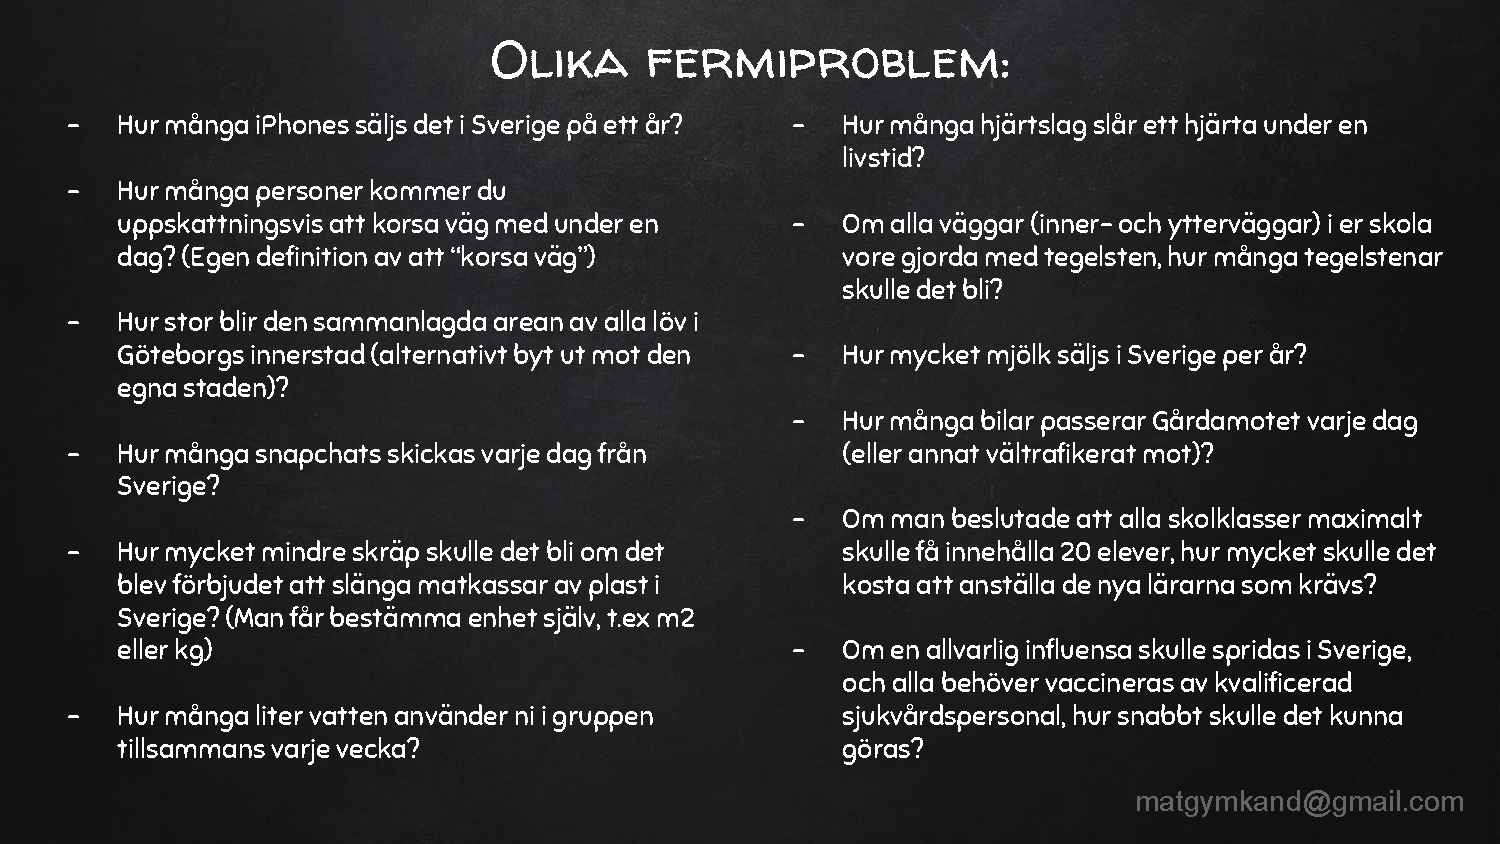
\includepdf{Appendix/Presentationer/Fermi.pdf}
    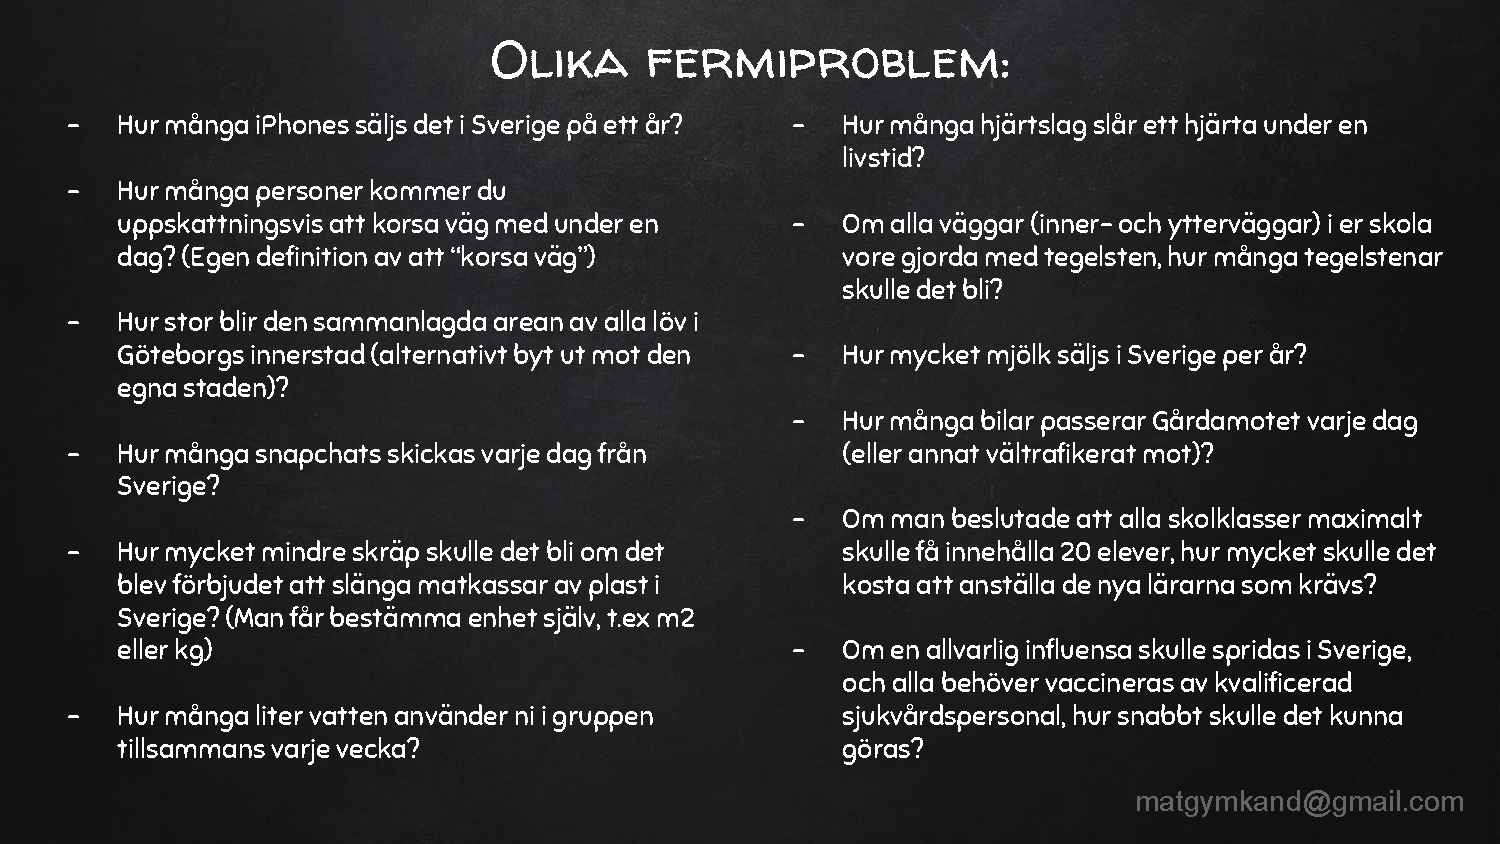
\includepdf[scale=0.9, pagecommand=\section{Presentationerna tillhörande problemen}\subsection{Fermiproblem}]{Appendix/Presentationer/Fermi.pdf}
    
    %\subsection{Flygplan}
    
\includepdf[scale=0.9,pagecommand=\subsection{Flygplan}]{Appendix/Presentationer/Flygplan.pdf}
    \includepdfmerge[nup=1x3] {Appendix/Presentationer/Flygplan.pdf, 2-4}
    \includepdfmerge[nup=1x3] {Appendix/Presentationer/Flygplan.pdf, 5-7}
    
    %\subsection{Fritt fall}
    
\includepdf[scale=0.9,pagecommand=\subsection{Fritt fall}]{Appendix/Presentationer/Frittfall.pdf}
    \includepdfmerge[nup=1x2, scale=0.9] {Appendix/Presentationer/Frittfall.pdf, 2-3}
    
    %\subsection{Försvåring av en ekvation}
    
\includepdf[scale=0.9,pagecommand=\subsection{Försvåring av en ekvation}]{Appendix/Presentationer/Ekvation.pdf}
    \includepdfmerge[nup=1x3] {Appendix/Presentationer/Ekvation.pdf, 2-4}
        
    %\subsection{Matematisk modell för bil och löpare}
    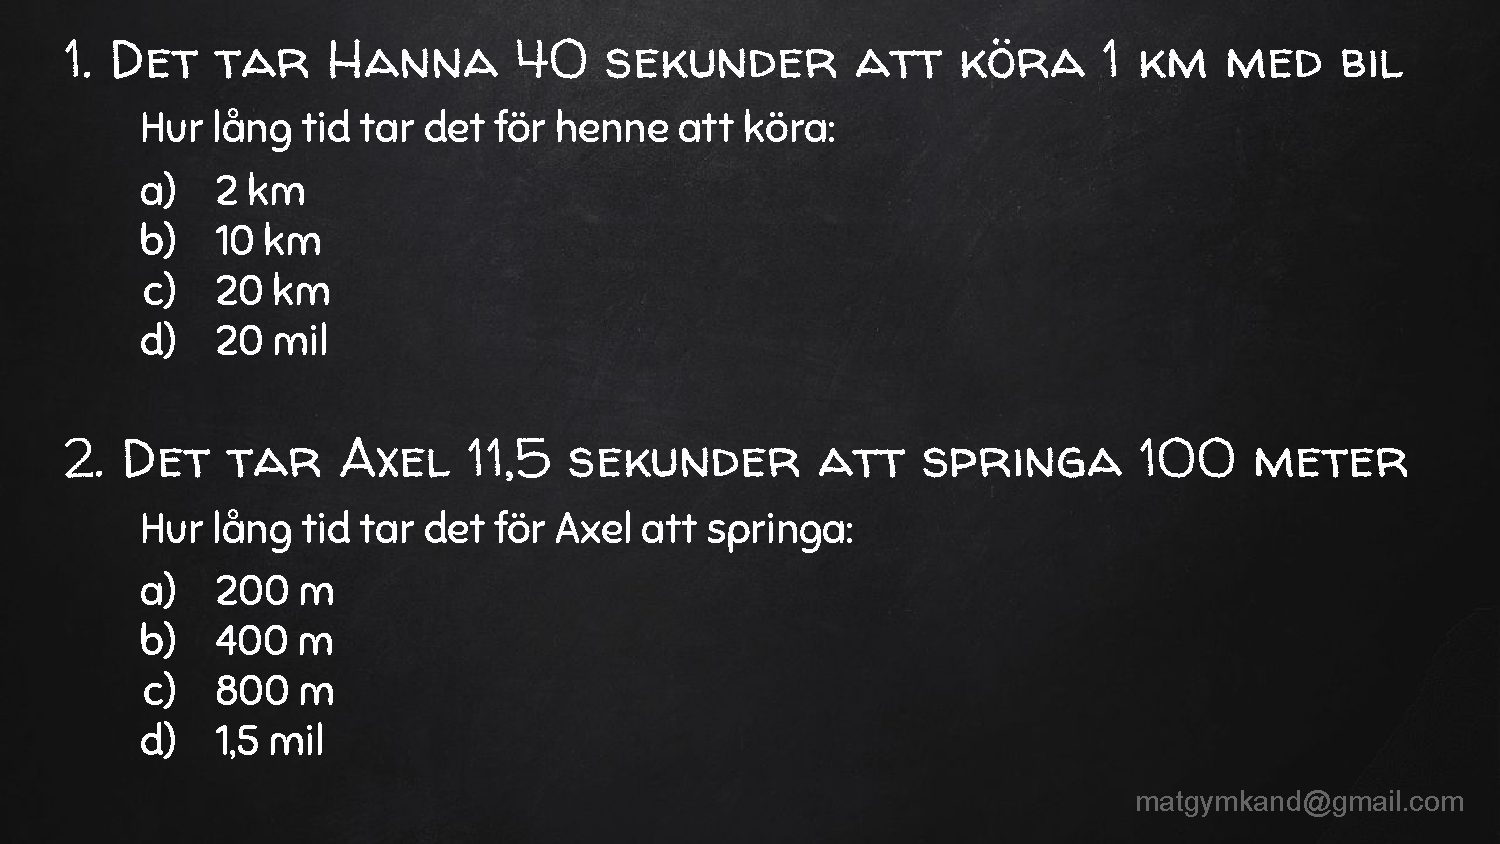
\includepdf[scale=0.9,pagecommand=\subsection{Matematisk modell för bil och löparen}]{Appendix/Presentationer/Lopare.pdf}
    \includepdfmerge[nup=1x2, scale=0.9] {Appendix/Presentationer/Lopare.pdf, 2-3}
    \includepdfmerge[nup=1x2, scale=0.9] {Appendix/Presentationer/Lopare.pdf, 4-5}
    
    %\subsection{Sortera en kortlek}
    
\includepdf[scale=0.9,pagecommand=\subsection{Sortera en kortlek}]{Appendix/Presentationer/Sortera.pdf}
        \includepdfmerge[nup=1x3] {Appendix/Presentationer/Sortera.pdf, 2-4}
        
    %\section{Enkäter}
    %\subsection{Förundersökning - Lärare}
    \includepdf[scale=0.9, pages=1, templatesize={180mm}{240mm}, noautoscale=true,  pagecommand=\section{Enkäter}\subsection{Förundersökning - Lärare}\label{sec:bakgrundsenkat}]{Appendix/Enkater/Forundersokning-Larare.pdf}
    \includepdf[pages=2]{Appendix/Enkater/Forundersokning-Larare.pdf}
    \includepdf[pages=3]{Appendix/Enkater/Forundersokning-Larare.pdf}
    
    %\subsection{Problemutvärdering - Lärare}
    \includepdf[scale=0.9, pages=1, templatesize={230mm}{150mm}, noautoscale=true, pagecommand=\subsection{Problemutvärdering - Lärare}]{Appendix/Enkater/Problemutvardering-Larare.pdf}
    \includepdf[pages=2]{Appendix/Enkater/Problemutvardering-Larare.pdf}
    \includepdf[pages=3]{Appendix/Enkater/Problemutvardering-Larare.pdf}
    \includepdf[pages=4]{Appendix/Enkater/Problemutvardering-Larare.pdf}
    
    %\subsection{Problemutvärdering - Elever}
    \includepdf[scale=0.9, pages=1, templatesize={230mm}{240mm}, noautoscale=true, pagecommand=\subsection{Problemutvärdering - Elever}]{Appendix/Enkater/Problemutvardering-Elever.pdf}
    \includepdf[pages=2]{Appendix/Enkater/Problemutvardering-Elever.pdf}
%    \includepdf[pages=3]{Appendix/Enkater/Problemutvardering-Elever.pdf}